\documentclass{beamer}
\usepackage[english]{babel}
\usepackage[utf8x]{inputenc}
\usepackage{graphicx}
\usepackage{tikz}

\usetheme{default}
\usecolortheme{default}
\usefonttheme{default}
\setbeamertemplate{caption}

\title{TeXpresso: live \LaTeX{} rendering}
\author{@let-def}
\date{\today}

\begin{document}

\begin{frame}
  \titlepage
\end{frame}

\begin{frame}{TeXpresso workflow}
  \begin{itemize}
   \item TeXpresso is a tool for previewing \LaTeX{} documents live.
    \item It supports Linux and macOS. \\
      {\small $\rightarrow$ Snapshotting is done using {\em fork(2)}.}
     \item It comes with an Emacs mode for live synchronisation. \\
     {\small $\rightarrow$ Alternatively, it detects changed files on SIGUSR1. \\ E.g. use \texttt{:!killall -SIGUSR1 texpresso} from vim.}
    \item It also reports \underline{errors and \hskip 0em warnings!}
  \end{itemize}
\end{frame}

\begin{frame}{Compatibility}
  \begin{itemize}
   \item Typesetting is done using a customized Tectonic \& XeTeX
   \item Rendering uses a custom DVI interpreter using MuPDF. \\
    Not perfect but quite compatible; e.g TikZ: \\
    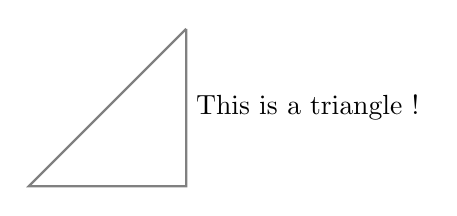
\begin{tikzpicture}
      \draw[gray, thick] (1,1) -- (-1,-1) -- (1,-1) -- (1,1);
      \filldraw[black] (1,0) node[anchor=west]{This is a triangle !};
    \end{tikzpicture}
   \item and Graphics: 
\includegraphics[scale=0.2]{../texpresso_logo.png}
   \item However, shell-escape is disabled! \\ (no live rendering of minted) :-(
  \end{itemize}
\end{frame}

\begin{frame}{Coming soon...}
  \begin{itemize}
    \item TeXpresso is slowly developed on my free time. \\
    \item I hope to have an alpha version, MIT-licensed, soon.
    \item Bonus: \textbf{dark mode} to take care of your fragile eyes \\
      \ldots and optional integration with \textbf{Emacs themes}.
  \end{itemize}
\end{frame}

\begin{frame}{That's all!}
  Thanks:
  \begin{itemize}
    \item to the developers of all free software that made this possible
    \item to the artists of the public-domain assets used in the logo!
    \item and to you for watching :-)
  \end{itemize}
\end{frame}

% \begin{frame}{Live edition}
%   TeXpresso is able to synchronize Emacs buffers in live.
%
%   This is the preferred workflow.
%
%   For other editors, it can efficiently reload files from the file system when receiving a SIGUSR1 signal.
% \end{frame}
%
% \begin{frame}{Live error report}
%   If you use Emacs, it is also able to report LaTeX error warnings in real-time.
%   Not a silver bullet, but convenient for debugging.
%   ThisIsNotAValid Command. Better :)
%
%   There is also a limited support for SyncTeX synchronization (but Beamer is not the best illustration of this feature!)
% \end{frame}
%
% \begin{frame}{Eye candy}
%   The renderer can use a dark mode, ... Or import an Emacs theme.
%   Not bad :).
% \end{frame}
% \section{Section Two}
%
% \begin{frame}{Slide with table}
% 	\input{tables/table1.tex}
% \end{frame}
%
% \begin{frame}{Slide with figure}
% 	\begin{figure}[H]
% 		\centering
%         \includegraphics[width=.5\textwidth]{figures/figure1.png}
%         \caption{Caption for figure one.}
%         \label{fig:figure1}
% 	\end{figure}
% \end{frame}
%
% \begin{frame}{Slide with references}
% 	This is to reference a figure (Figure \ref{fig:figure1})\\
%     This it to reference a table (Table \ref{tab:table1})\\
%     This is to cite an article \cite{Ahmed2018a}\\
%     This is to add an article to the references without mentioning in the text \nocite{Ahmed2018a}\\
% \end{frame}
% \section{References}
%
% % Adding the option 'allowframebreaks' allows the contents of the slide to be expanded in more than one slide.
% \begin{frame}[allowframebreaks]{References}
% 	\tiny\bibliography{references}
% 	\bibliographystyle{apalike}
% \end{frame}

\end{document}
